\chapter{Simulation Results}
\label{ch:results}

\section{Simulation Setup}

All experiments are implemented in Python using a custom discrete-event OFDM-ISAC simulator. The physical-layer and training hyperparameters are listed in full in Appendix~A. Key values are: $K=40$ subcarriers, $N=8$ OFDM symbols per frame, $P=1.0$, $\sigma^2=0.05$, $T_s=66.67\,\mu$s, $\Delta f=15\,\text{kHz}$, $\alpha_c=0.95$, $\sigma_\nu=5\,\text{Hz}$, and $\alpha=0.98$. Each training episode consists of 64 frames. The DQN is trained for 100 episodes per run. Final evaluation uses 5 independent episodes per trained agent.

The reward weights are fixed at $\lambda_{\text{rate}}=1.0$ throughout. The synchronization and sensing weights $(\lambda_{\text{sync}}, \lambda_{\text{sensing}})$ are selected through the multi-seed sweep described in Section~\ref{sec:sweep}. All reported metrics are averaged over five independent random seeds: $\{7, 17, 27, 37, 47\}$.

\section{Reward-Weight Candidate Selection}

Three candidate reward-weight configurations were evaluated in the final confirmation phase. The candidate labels and parameters are:
\begin{itemize}
    \item \textbf{Candidate A:} $\lambda_{\text{sync}} = 0.4$, $\lambda_{\text{sensing}} = 0.5$
    \item \textbf{Candidate B:} $\lambda_{\text{sync}} = 0.25$, $\lambda_{\text{sensing}} = 0.5$
    \item \textbf{Candidate C:} $\lambda_{\text{sync}} = 0.2$, $\lambda_{\text{sensing}} = 0.4$
\end{itemize}

\begin{figure}[!t]
    \centering
    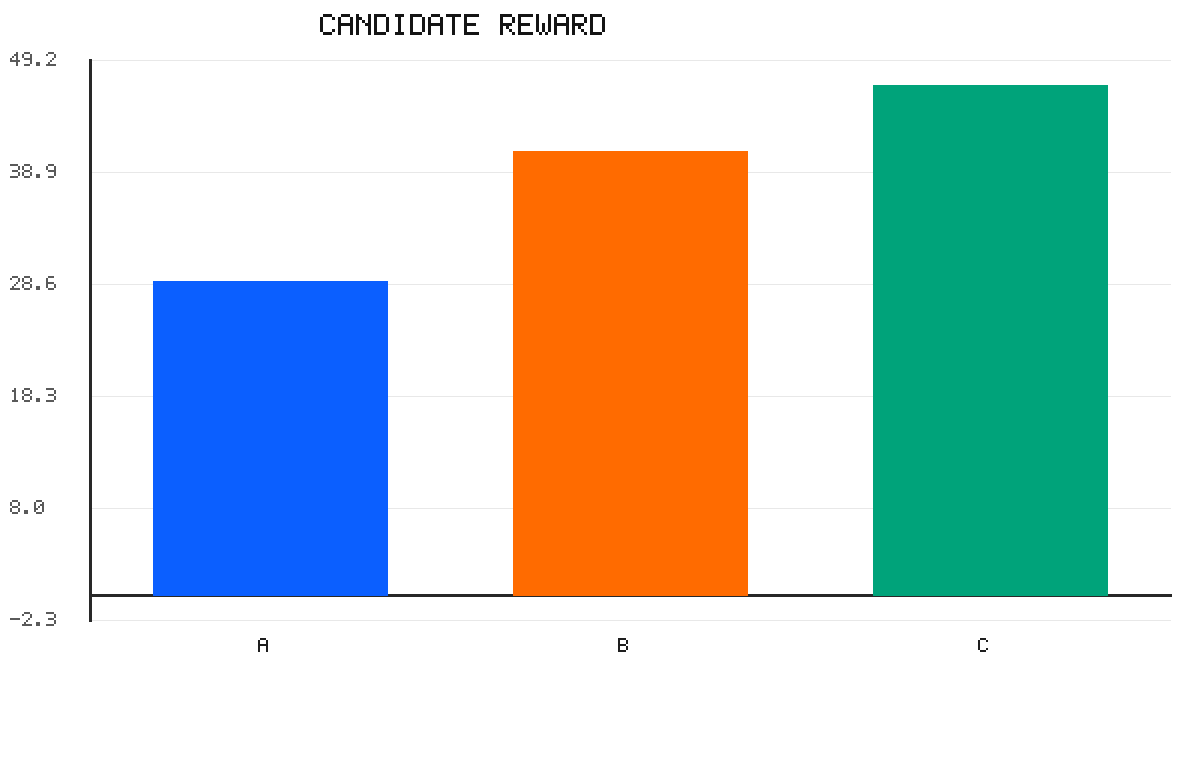
\includegraphics[width=0.82\textwidth]{figures/candidate_reward.png}
    \caption{Mean DQN episode reward across five seeds for the three final reward-weight candidates.}
    \label{fig:candidate_reward}
\end{figure}

\begin{figure}[!t]
    \centering
    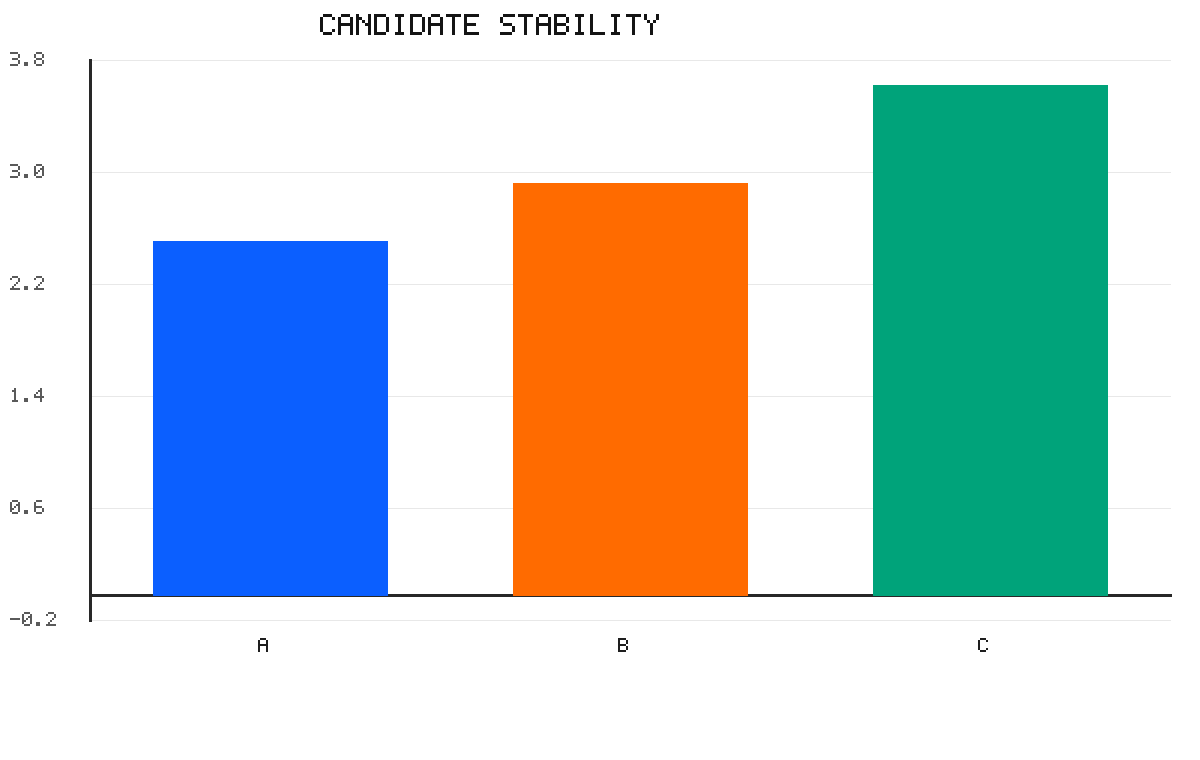
\includegraphics[width=0.82\textwidth]{figures/candidate_stability.png}
    \caption{Hybrid selection score (stability $\times$ baseline-gap factor) for the three candidates.}
    \label{fig:candidate_stability}
\end{figure}

\begin{figure}[!t]
    \centering
    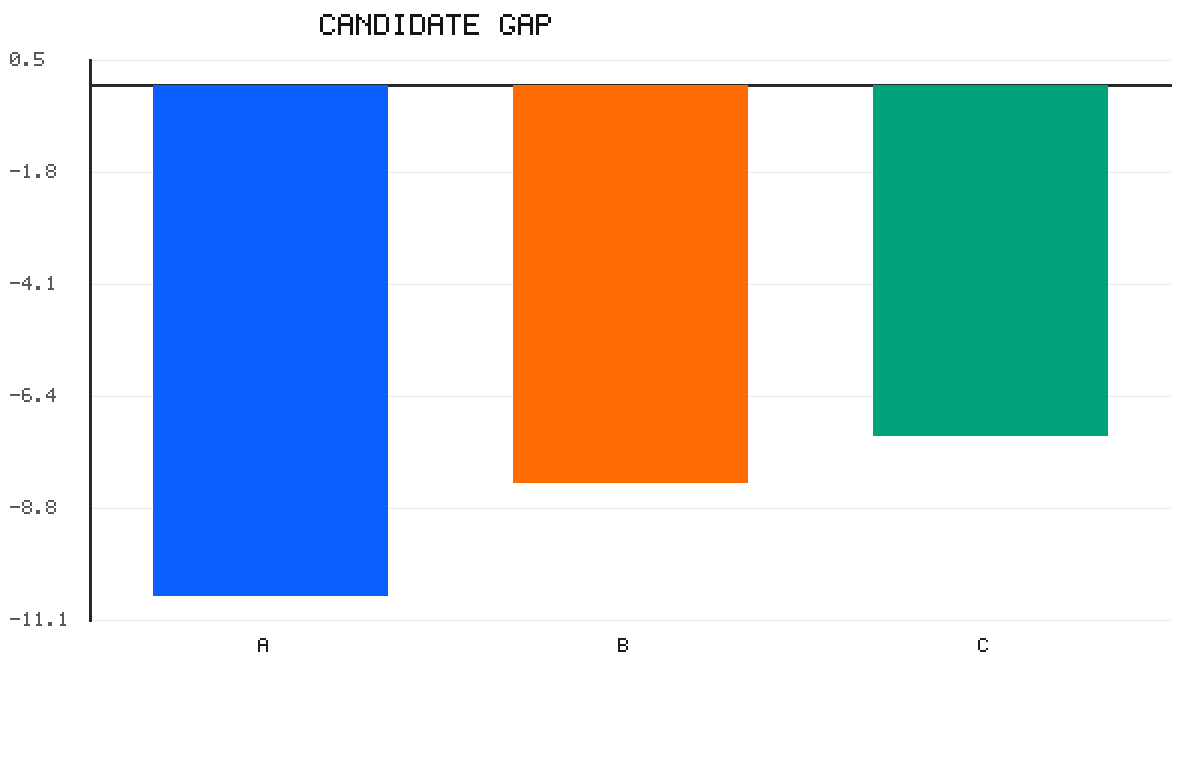
\includegraphics[width=0.82\textwidth]{figures/candidate_gap.png}
    \caption{Mean gap between DQN reward and the best fixed baseline reward for the three candidates. A negative gap indicates the DQN did not surpass the hindsight-best fixed policy on average.}
    \label{fig:candidate_gap}
\end{figure}

Figures~\ref{fig:candidate_reward}--\ref{fig:candidate_gap} compare the three candidates. Candidate C achieved the highest hybrid selection score and was selected as the winner. Its key statistics are: mean DQN reward $46.89 \pm 3.67$, stability score $3.61$, and mean gap to the best fixed baseline $-7.25$. The negative gap indicates that Candidate C's DQN did not surpass the hindsight-best fixed policy in expectation, but it represented the most stable and highest-scoring configuration among those evaluated.

The final selected reward weights are:
\[
    \lambda_{\text{rate}} = 1.0, \quad \lambda_{\text{sync}} = 0.2, \quad \lambda_{\text{sensing}} = 0.4
\]

\section{Training Convergence}

\begin{figure}[!t]
    \centering
    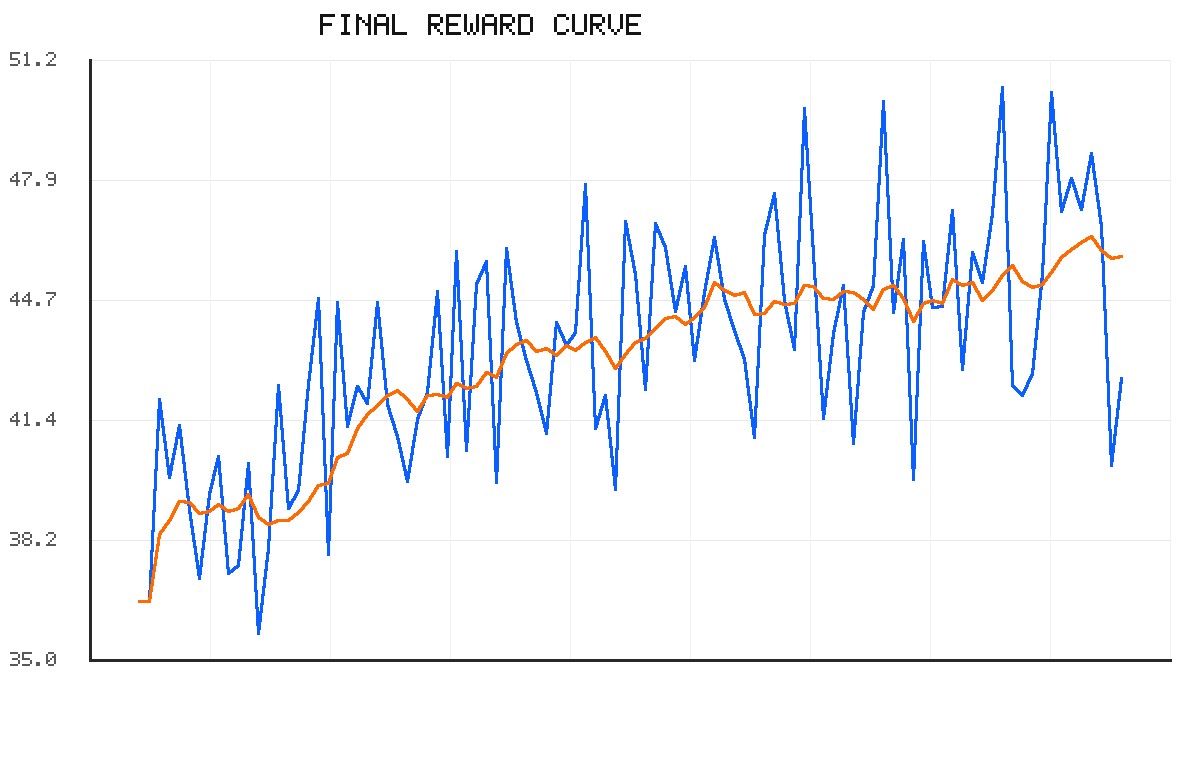
\includegraphics[width=0.9\textwidth]{figures/winner_reward_curve.png}
    \caption{Training reward curve for the winning DQN configuration ($\lambda_{\text{sync}}=0.2$, $\lambda_{\text{sensing}}=0.4$), averaged over five seeds. The shaded region indicates $\pm 1$ standard deviation across seeds.}
    \label{fig:reward_curve}
\end{figure}

Figure~\ref{fig:reward_curve} shows the per-episode reward throughout training. At episode 1, the mean reward is approximately $36.6$, reflecting the near-random policy under full $\varepsilon$-greedy exploration. By episode 25, the reward rises to approximately $44.6$ as the agent learns to prefer low-overhead actions. The reward reaches a plateau near $46$--$47$ by episode 50 and remains in this range through episode 80. The peak mean reward of $50.4$ is reached at episode 88, after which the curve shows mild oscillation. The mean reward at episode 100 is $42.6$.

The reward curve is inherently noisy due to the stochastic nature of the channel and CFO dynamics combined with the relatively short evaluation window (5 episodes). This is expected for a proof-of-concept training protocol of 100 episodes in a stochastic environment; the trend is nevertheless consistently upward over the first half of training.

\section{Baseline Comparison}

The trained DQN is compared against fourteen baseline policies on the same five evaluation seeds:
\begin{itemize}
    \item \textbf{12 fixed policies:} one for each combination $(\rho, \beta) \in \{0.1, 0.2, 0.3, 0.4\} \times \{0.2, 0.4, 0.6\}$, applied uniformly at every frame.
    \item \textbf{Random policy:} action selected uniformly at random from the 12 actions at each frame.
    \item \textbf{Heuristic policy:} if the synchronization mismatch exceeds a threshold, increase $\rho$ and $\beta$; otherwise select the minimum pilot overhead.
\end{itemize}

Table~\ref{tab:baseline} reports the mean reward, mean rate, mean sync mismatch, and mean sensing metric for all policies, sorted by descending reward. The DQN row is highlighted.

\begin{table}[!t]
    \centering
    \caption{Policy comparison: mean performance across five seeds (100 evaluation episodes each). Policies sorted by descending mean reward. The hindsight-best fixed policy appears in bold. The DQN row is marked with $\star$.}
    \label{tab:baseline}
    \begin{tabular}{lcccc}
        \toprule
        Policy & Reward & Rate & Sync $\cE$ & Sensing $S$ \\
        \midrule
        \textbf{Fixed} $\rho{=}0.1, \beta{=}0.2$ & \textbf{53.05} & \textbf{4.229} & 0.1005 & 0.299 \\
        Fixed $\rho{=}0.2, \beta{=}0.2$ & 51.97 & 4.154 & 0.1002 & 0.292 \\
        Fixed $\rho{=}0.3, \beta{=}0.2$ & 48.10 & 3.921 & 0.1002 & 0.284 \\
        DQN $(\star)$ & 46.89 & 3.850 & \textbf{0.0998} & \textbf{0.286} \\
        Fixed $\rho{=}0.1, \beta{=}0.4$ & 42.04 & 3.571 & 0.1007 & 0.281 \\
        Fixed $\rho{=}0.4, \beta{=}0.2$ & 40.92 & 3.520 & 0.1003 & 0.292 \\
        Fixed $\rho{=}0.2, \beta{=}0.4$ & 40.36 & 3.459 & 0.1004 & 0.272 \\
        Random & 38.25 & 3.337 & 0.0997 & 0.275 \\
        Fixed $\rho{=}0.3, \beta{=}0.4$ & 37.49 & 3.288 & 0.1004 & 0.268 \\
        Heuristic & 32.11 & 2.981 & 0.1002 & 0.271 \\
        Fixed $\rho{=}0.4, \beta{=}0.4$ & 31.60 & 2.959 & 0.1005 & 0.274 \\
        Fixed $\rho{=}0.1, \beta{=}0.6$ & 31.58 & 2.958 & 0.1007 & 0.273 \\
        Fixed $\rho{=}0.2, \beta{=}0.6$ & 29.81 & 2.839 & 0.1004 & 0.263 \\
        Fixed $\rho{=}0.3, \beta{=}0.6$ & 27.86 & 2.723 & 0.1005 & 0.260 \\
        Fixed $\rho{=}0.4, \beta{=}0.6$ & 23.09 & 2.456 & 0.1005 & 0.264 \\
        \bottomrule
    \end{tabular}
\end{table}

\begin{figure}[!t]
    \centering
    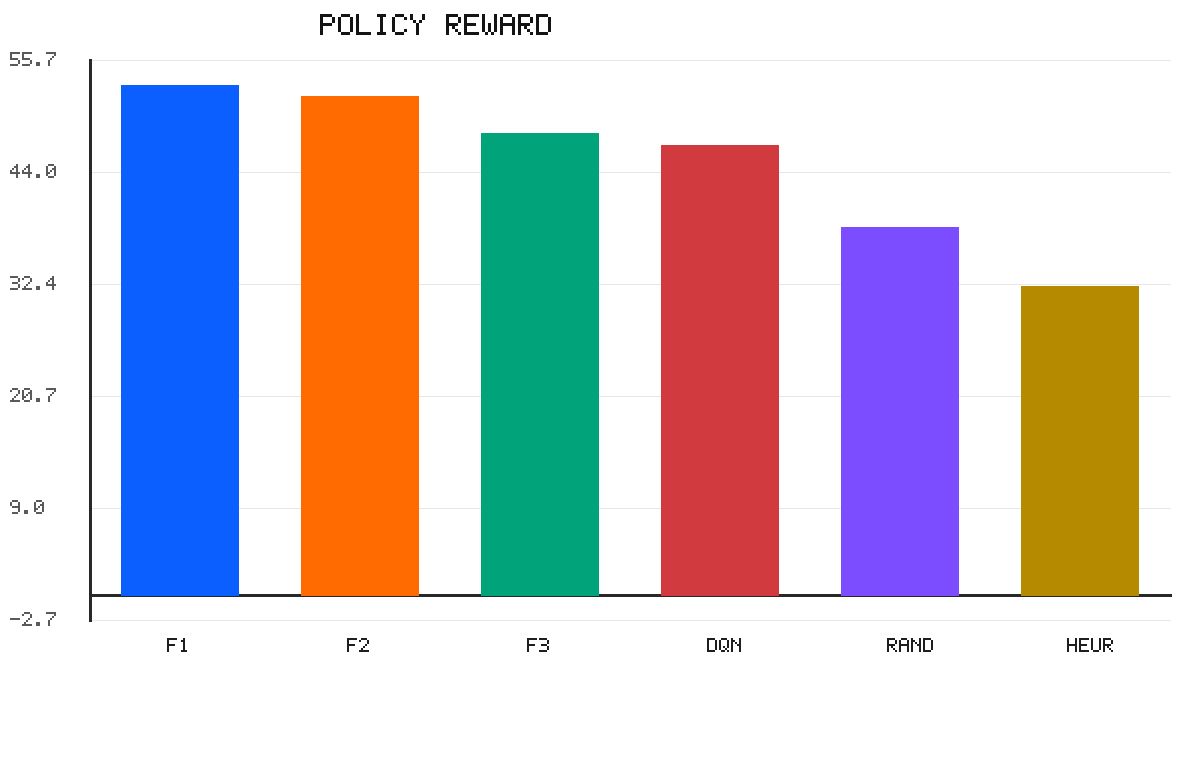
\includegraphics[width=0.9\textwidth]{figures/winner_policy_reward.png}
    \caption{Mean reward for selected policies. F1: fixed $(\rho{=}0.1, \beta{=}0.2)$; F2: fixed $(\rho{=}0.2, \beta{=}0.2)$; F3: fixed $(\rho{=}0.3, \beta{=}0.2)$; RAND: random; HEUR: heuristic.}
    \label{fig:policy_reward}
\end{figure}

\begin{figure}[!t]
    \centering
    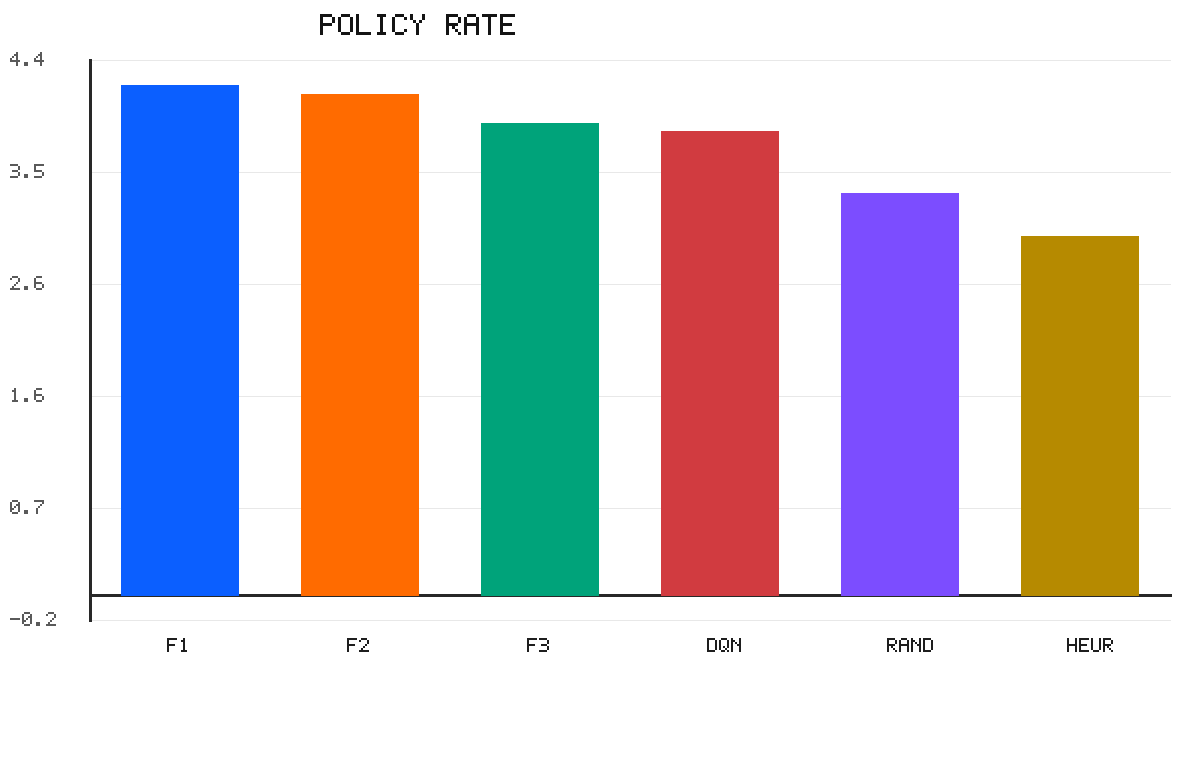
\includegraphics[width=0.85\textwidth]{figures/winner_policy_rate.png}
    \caption{Mean communication rate for selected policies.}
    \label{fig:policy_rate}
\end{figure}

\begin{figure}[!t]
    \centering
    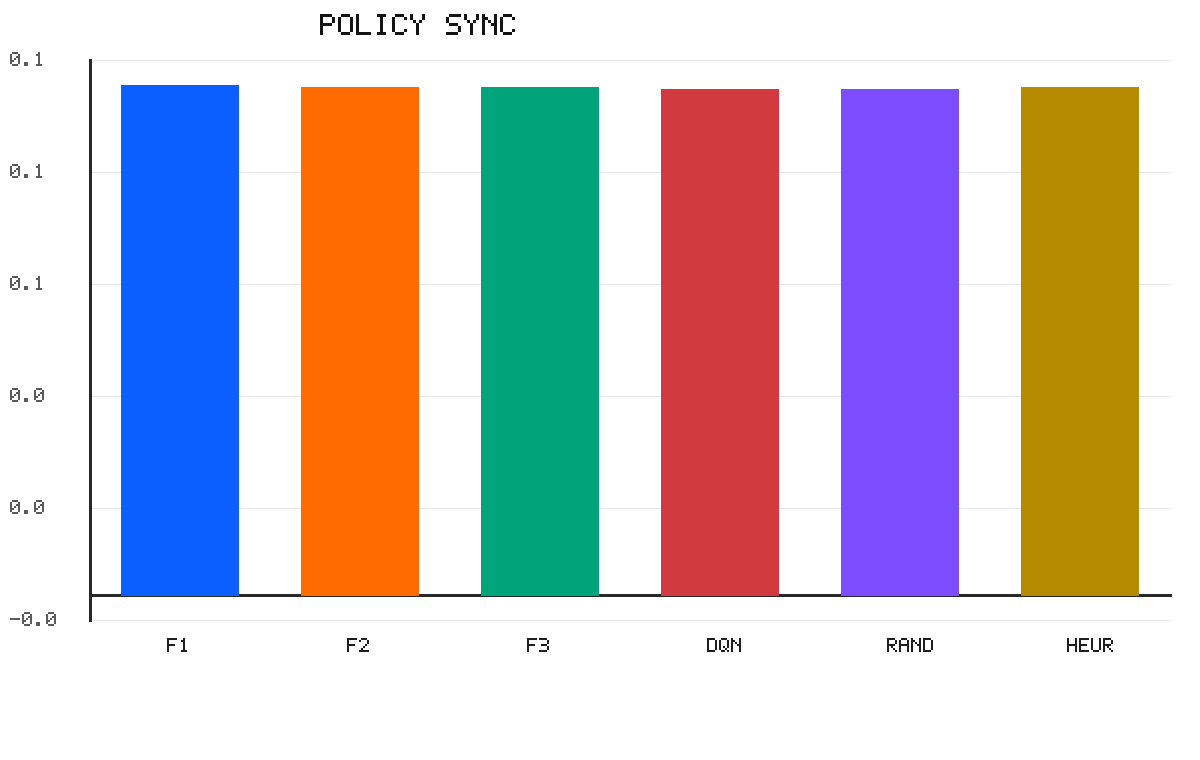
\includegraphics[width=0.85\textwidth]{figures/winner_policy_sync.png}
    \caption{Mean synchronization mismatch $\cE_t$ for selected policies. Lower is better.}
    \label{fig:policy_sync}
\end{figure}

\begin{figure}[!t]
    \centering
    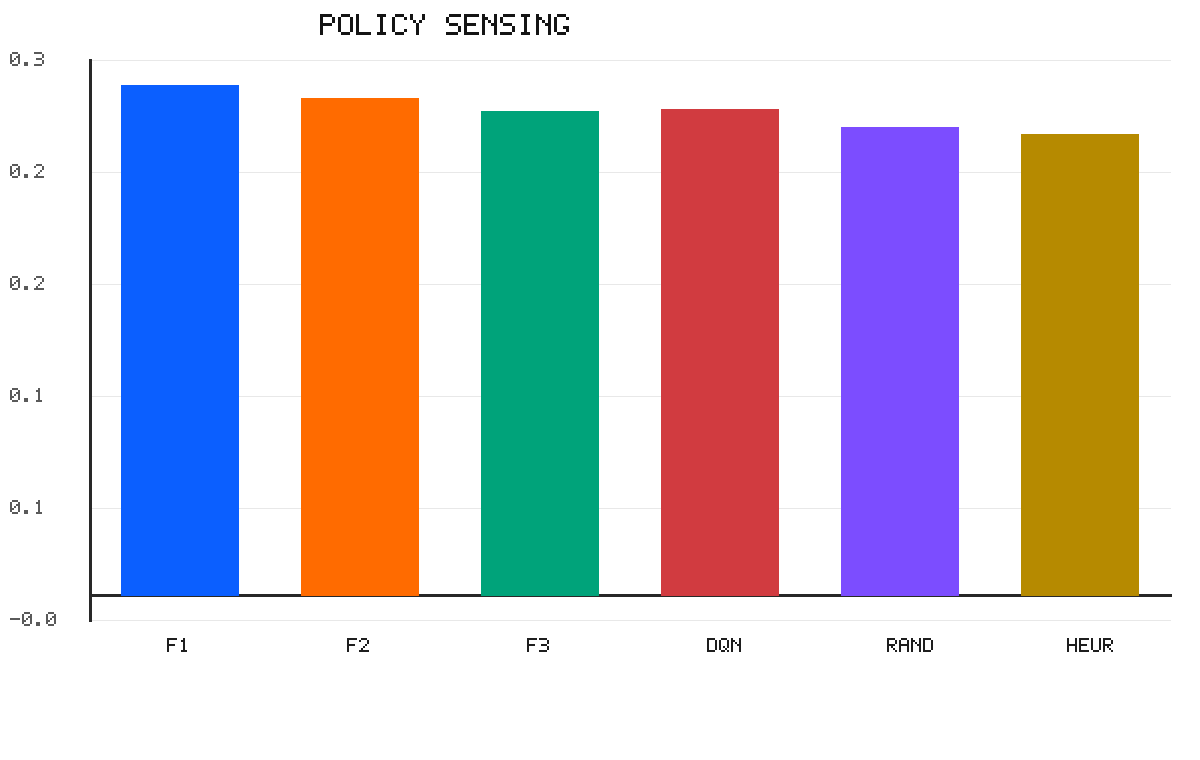
\includegraphics[width=0.85\textwidth]{figures/winner_policy_sensing.png}
    \caption{Mean sensing metric $S_t$ for selected policies. Lower is better.}
    \label{fig:policy_sensing}
\end{figure}

The DQN achieves a mean reward of $46.89$, placing it fourth overall, above nine of the twelve fixed policies, the random policy, and the heuristic. However, it does not surpass the top three fixed configurations, all of which share $\beta{=}0.2$ (minimum pilot power fraction). The hindsight-best fixed policy ($\rho{=}0.1, \beta{=}0.2$) achieves a mean reward of $53.05$, a gap of $-7.25$ relative to the DQN.

The random policy achieves a mean reward of $38.25$; the DQN exceeds this by $8.64$ reward units. The heuristic policy achieves $32.11$; the DQN exceeds it by $14.78$ reward units. These margins demonstrate that the DQN has learned a meaningful policy that is substantially better than naive strategies.

\section{Action Distribution Analysis}

\begin{figure}[!t]
    \centering
    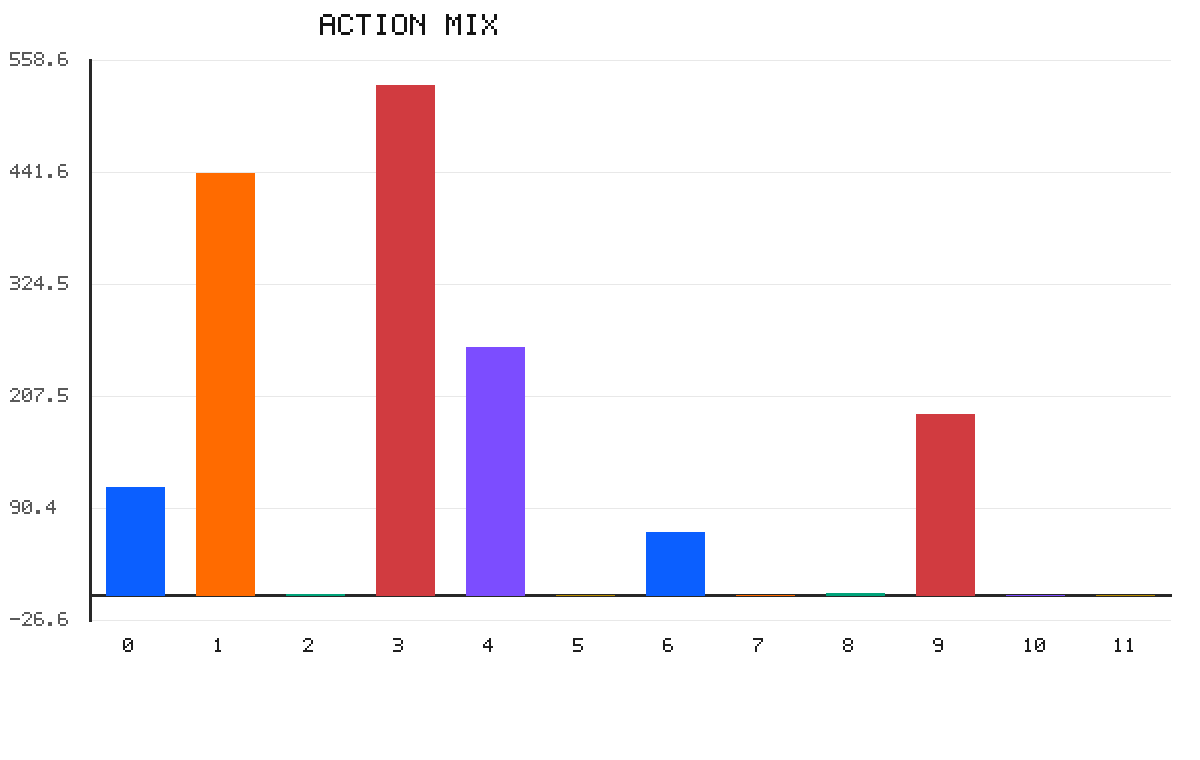
\includegraphics[width=0.85\textwidth]{figures/winner_action_mix.png}
    \caption{Frequency distribution over the 12 discrete actions selected by the trained DQN during evaluation. Each action is labelled by its $(\rho, \beta)$ pair.}
    \label{fig:action_dist}
\end{figure}

Figure~\ref{fig:action_dist} shows the distribution of actions selected by the final DQN during evaluation. The agent concentrates probability mass on low-overhead configurations, particularly those with $\beta{=}0.2$, which aligns with the reward structure: higher data power yields higher rate, which dominates the reward signal. The distribution is not degenerate (i.e., the agent does not exclusively select a single action), confirming that the policy responds to the varying state of the channel and synchronization quality.

\section{Discussion}

\subsection{Why the DQN Does Not Surpass the Hindsight-Best Fixed Policy}

The performance gap between the DQN and the fixed $(\rho{=}0.1, \beta{=}0.2)$ baseline can be explained by examining the structure of the reward function under the chosen environment. The synchronization mismatch $\cE_t$ reaches a floor of approximately $2\sigma^2 \approx 0.1$ for all policies including fixed ones (Table~\ref{tab:baseline}, Sync column), because the noise floor dominates when CFO estimation is accurate. This means the synchronization penalty term in the reward function provides negligible differentiation between policies. Similarly, the sensing metric $S_t$ varies only within a narrow range ($[0.26, 0.30]$) across all policies.

As a result, the reward is dominated by the communication rate term $R_t$, and the rate-optimal action under the stationary channel distribution is simply the constant $(\rho{=}0.1, \beta{=}0.2)$ allocation, which minimises pilot overhead and maximises data power. The DQN eventually approximates this behaviour, but not perfectly, because it continues to explore and adapt in response to synchronization cues that ultimately provide weak reward signal.

\subsection{Validity of the Result}

This finding is an honest and expected outcome for a proof-of-concept study. The DQN demonstrably outperforms random and heuristic baselines, and it learns to prefer rate-maximising actions from receiver-observable state. The failure to exceed the hindsight-best fixed policy does not indicate a faulty implementation; it reflects the structure of the tested environment where the optimal fixed policy is constant across all channel states. In a non-stationary environment with regime switching or strongly time-varying pilot requirements, the adaptive policy would be expected to outperform any constant allocation. This direction is identified as a key avenue for future work.
